\clearpage
\section{Stromové kódy}
\subsection{Popište základní vlastnosti stromových kódů a odlišnost oproti blokovým.}
Stromové kódy mají jiný způsob zabezpečení datového toku v porovnání s kódy blokovými. 
Dalším prvkem zabezpečení zde, krom vkládání nadbytečných prvků, je jejich závislost na předchozích 
informačních prvcích nezabezpečeného datového toku. \\
Parametry:
\begin{itemize}
    \item $k_0$ počet bitů ve vstupním bitovém úseku
    \item $n_0$ počet bitů ve výstupním bitovém úseku
    \item informační rychlost $R=\frac{k_0}{n_0}$
    \item délka kódového ohraničení $\nu=m\cdot k_0$ (viz. \ref{nu})
    \item Nezabezpečený blok stromového kódu $k=(m+1)\cdot k_0$
    \item Zabezpečený blok stromového kódu $n=(m+1)\cdot n_0$
\end{itemize}


\subsection{Vysvětlete zadávání konvolučních kódů vytvářecími mnohočleny.}
Používáme operátor zpoždění $D$, jednotlivé mnohočleny mají v horním indexu vstupní tok, v dolním výstupní tok.
Znázorňují vazbu mezi vstupy a výstupy pomocí operátoru zpoždění. Příklady:
\begin{itemize}
    \item $G^{(i)}_{(j)}(D)$ - obecný zápis
    \item $G^{(1)}_{(1)}(D)=1+D$, $G^{(1)}_{(2)}(D)=1+D^2$ apod.
\end{itemize} 

\subsection{Vysvětlete zadávání konvolučních kódů vytvářecími maticemi.}
Vstupní toky jsou řádky matice $P$, výstupní pak $F$, vytvářecí matice je $G$. Platí $F=P\cdot G$. $G$ je
polonekonečná, protože je ohraničená délkou zprávy, která teoreticky může být i nekonečná. $G\infty$ 
se skládá z dílčích vytvářecích matic $G_t$, které mají $k$ řádků a $n$ sloupců. $G$ Umožňuje přepočítat sloupec 
vstupní matice $P$ pro časový okamžik $t$ na sloupec výstupní matice $F$ pro stejný časový okamžik. Ze vztahu (8.11) je zřejmé, že k popisu kódu pomocí $G\infty$ nám stačí znát sestavu matic $G_t$ pro $t = 1, 2, \dots, m$. \\
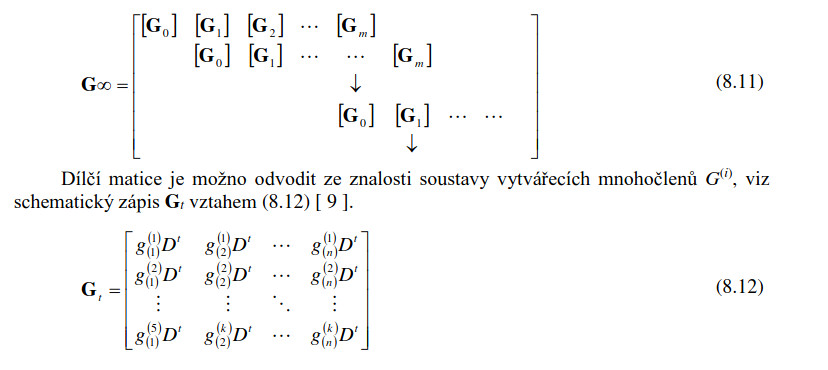
\includegraphics[width=16cm]{images/8_matice.png} \\
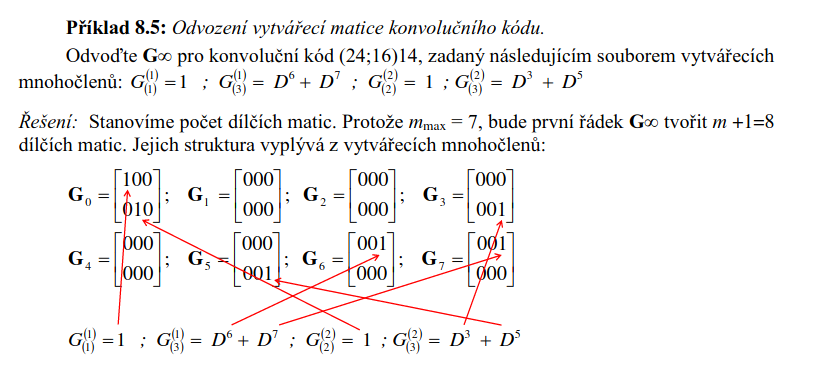
\includegraphics[width=16cm]{images/8_odvozeni.png}

\subsection{Vysvětlete princip a popište stromový graf.}
Graf znázorňuje vstupní bit, hodnoty pamětí a výstupní posloupnosti.\\
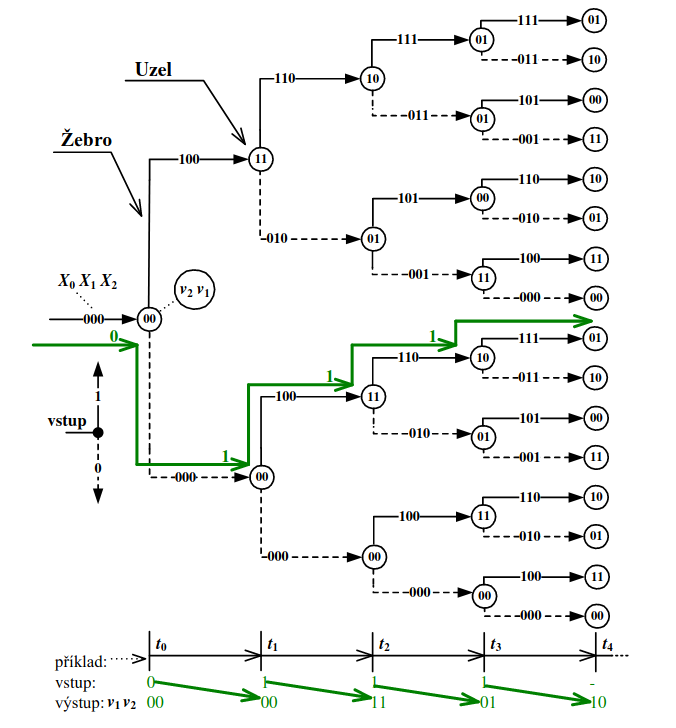
\includegraphics[width=16cm]{images/8_strom.png}

\subsection{Vysvětlete princip a popište mřížový graf.}
Podobný jako stromový, nerozvíjí se do nekonečna, ale opakuje se, když jsou v paměti všechny možnosti. \\
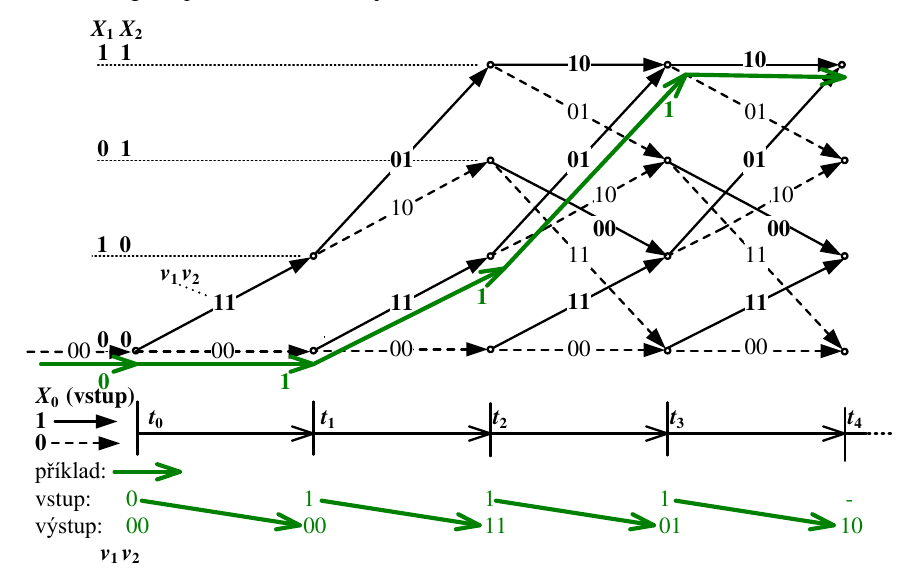
\includegraphics[width=16cm]{images/8_mriz.png}

\subsection{Vysvětlete princip a popište stavový diagram.}
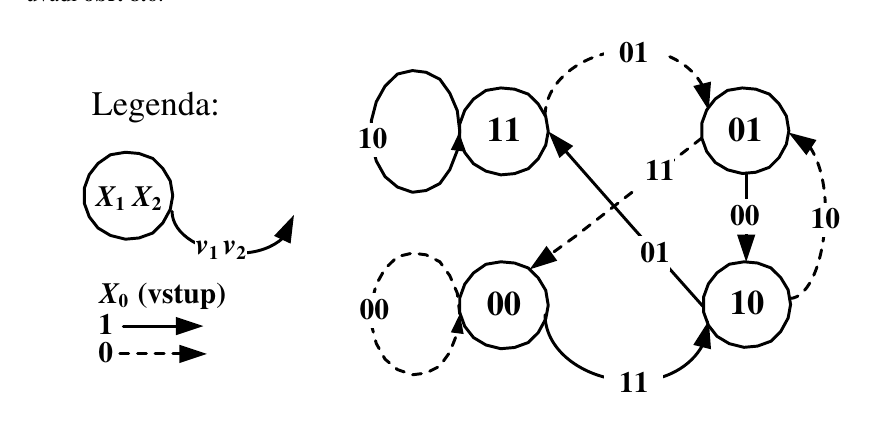
\includegraphics[width=16cm]{images/8_stav.png}

\subsection{Vysvětlete princip prahového dekódování konvolučního kódu.}
\begin{itemize}
    \item = syndromové dekódování
    \item Kontrolní matice $H\infty$ slouží k nalezení syndromu $s\infty$
    \item Kontrolní proces: $H\infty\cdot j\infty^T=s\infty^T$
    \item proces:
    \begin{itemize}
        \item Převedení sériového vstupu na paralelní
        \item Rozdělení na informační a zabezpečovací bity každého paralelně uspořádaného úseku
        \item Z informačních bitů se odvodí nové zabezpečovací bity a porovnají se s přijatými v generátoru syndromu
        \item Pokud došlo při přenosu k chybě, syndrom obsahuje informace o její poloze.
    \end{itemize}
\end{itemize}
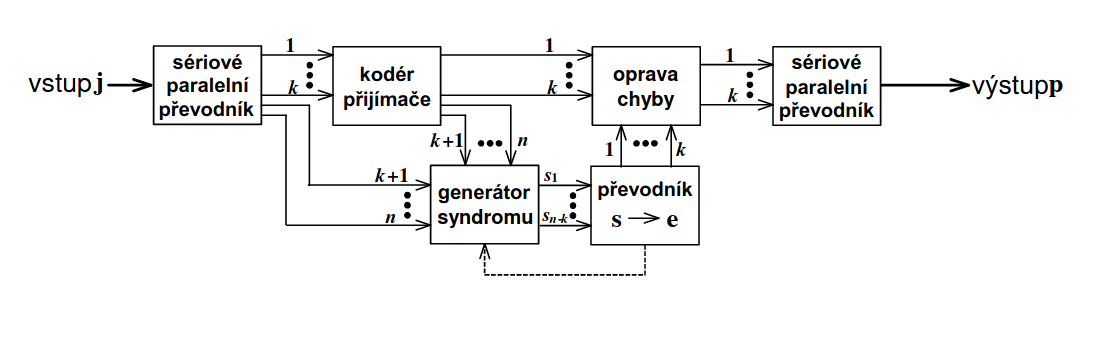
\includegraphics[width=16cm]{images/8_syndromove.png}

\subsection{Vysvětlete princip postupného pravděpodobnostního dekódování konvolučního kódu.}
\begin{itemize}
    \item Porovnává přijatou zprávu se seznamem užívaných zpráv a hledá nejmenší odchylku.
    \item Vhodná vizualizace procesu je dekódování pomocí mřížového grafu.
    \item Vzdálenost nejpravděpodobnější možnosti a přijatou zprávou je tzv. \textit{cena cesty}.
    \item U binárních kódů odpovídá cena cesty Hammingově vzdálenosti.
    \item typy:
    \begin{itemize}
        \item Postupné dekódování - o správnosti se rozhoduje prvek po prvku
        \item Dekódování po úsecích - o správnosti se rozhoduje po úsecích, Viterbiho algoritmus
    \end{itemize}
\end{itemize}

\subsection{Vysvětlete princip Viterbiho dekódovacího algoritmu.}
\begin{itemize}
    \item Po úsecích
    \item Úseky jsou porovnávány s používanými úseky v mřížovém grafu.
    \item Vybere se cesta s nejmenší cenou, z ní se odvodí informační prvky.
    \item Ochranná dekódovací hloubka $\mu$ by měla být 4 až 5 násobek kódového ohraničení $\nu$
    \item To, co jsme dělali v počítačových cvičeních
\end{itemize}

\subsection{Co je to délka kódového ohraničení $\nu$? Jaká je souvislost této délky a ochranné
dekódovací hloubky, při využití Viterbiho diagramu?} \label{nu}
\begin{itemize}
    \item Vyjadřuje, jak dlouho se bit podílí na zabezpečovacím procesu, vyjádřeno v bitech.
    \item Také určuje počet paměťových buněk paměti zabezpečovacího zařízení.
    \item Nezabezpečený blok stromového kódu $k$ je větší o 1 blok $k_0$, protože se na tvorbě podílí jeden 
    neuložený blok navíc.
    \item Z důvodu spolehlivosti by měla být u Viterbiho algoritmu ochranná dekódovací hloubka $\mu$
    4 až 5 násobek kódového ohraničení $\nu$.
\end{itemize}